
Эндээс бид системийн дарааллын загварыг тодорхойлж, хэрэглэгчдийн (Админ, Менежер, Ажилтан) системтэй харилцах үйл явцыг харуулна.

\subsection*{Загварын Тойм}
Дарааллын загвар нь хэрэглэгчийн үйлдэл, Next.js интерфэйс, Golang API, PostgreSQL мэдээллийн сан хоорондын харилцан үйлчлэлийг цаг хугацааны дарааллаар дүрсэлнэ. Доорх диаграммууд нь тус тусын дүрийн онцлог үйлдлүүдийг харуулна.

\subsection*{Админы Дарааллын Диаграмм}
Дарааллын диаграмм нь админы нэвтрэх, хэрэглэгч бүртгэх, системийн лог харах үйл явцыг харуулна.
\begin{figure}[H]
    \centering
    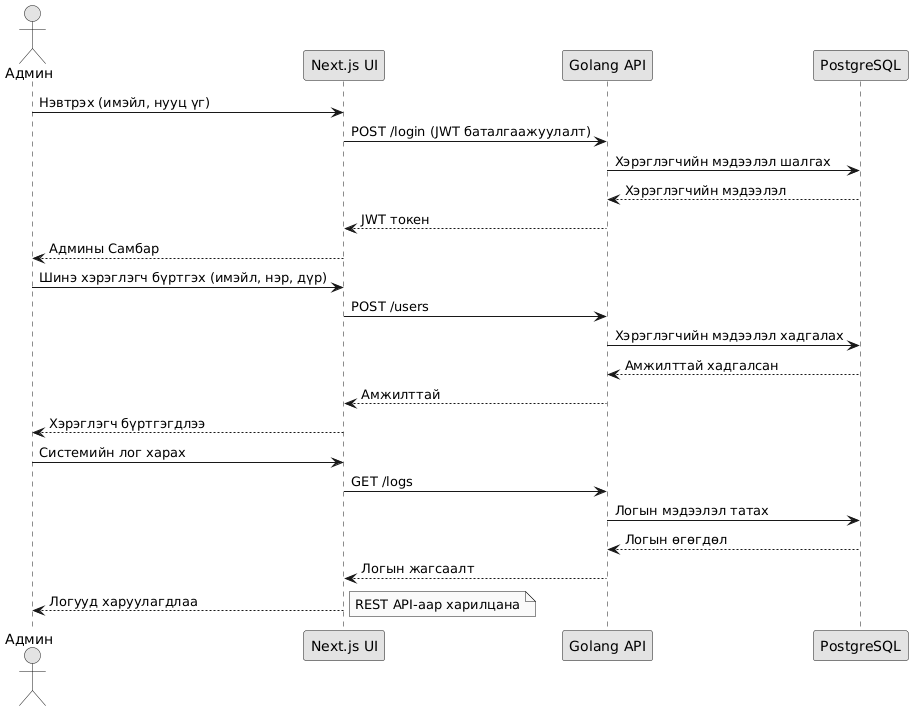
\includegraphics[width=\textwidth]{src/images/admin-seq.png}
    \caption{Админы Дарааллын Диаграм}
    \label{fig:admin_sequence_diagram}
\end{figure}

\subsection*{Менежерын Дарааллын Диаграмм}
Дарааллын диаграмм нь менежерын нэвтрэх, даалгавар хуваарилах, гүйцэтгэлийг үнэлэх үйл явцыг харуулна.
\begin{figure}[H]
    \centering
    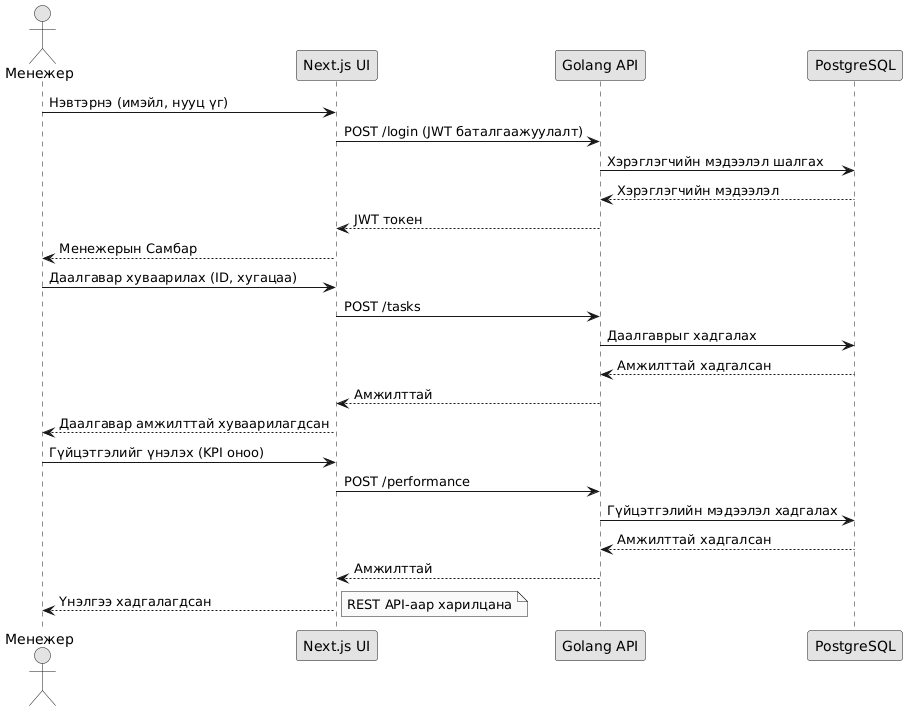
\includegraphics[width=\textwidth]{src/images/manager_seq.png}
    \caption{Менежерын Дарааллын Диаграм}
    \label{fig:manager_sequence_diagram}
\end{figure}

\subsection*{Ажилтны Дарааллын Диаграмм}
Дарааллын диаграмм нь ажилтны нэвтрэх, хуваарилагдсан даалгаврыг харах, статусыг шинэчлэх үйл явцыг харуулна.
\begin{figure}[H]
    \centering
    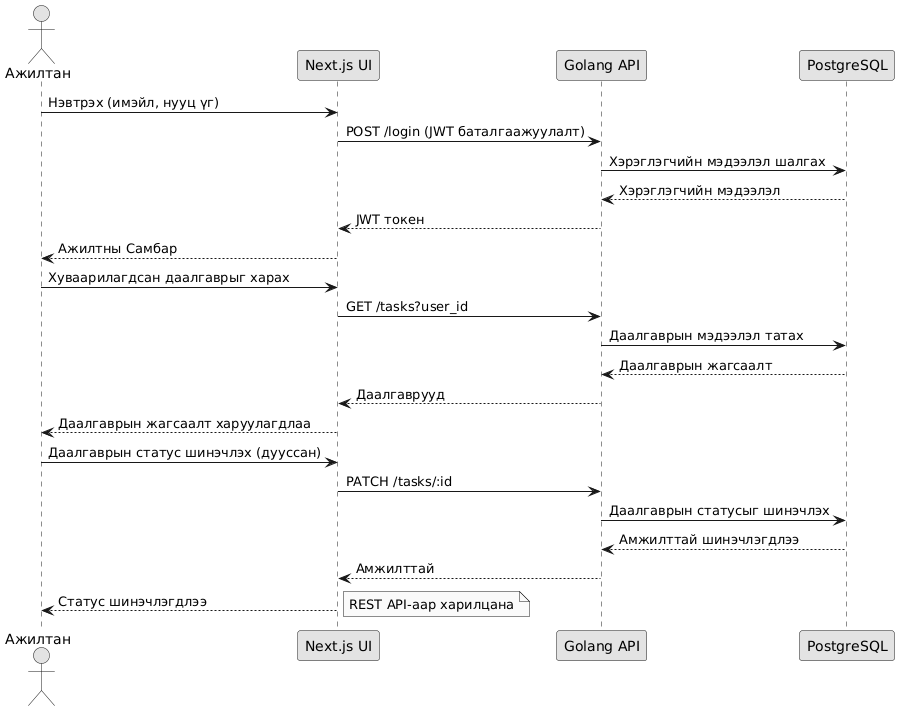
\includegraphics[width=\textwidth]{src/images/employee_seq.png}
    \caption{Ажилтны Дарааллын Диаграм}
    \label{fig:employee_sequence_diagram}
\end{figure}

\textbf{Тайлбар:} Эдгээр диаграммууд нь REST API-аар дамжуулан Next.js UI, Golang API, PostgreSQL хоорондын харилцан үйлчлэлийг тодорхойлж, хэрэглэгч тус бүрийн үндсэн үйлдлүүдийг харуулсан болно.